%-----------------------------------------------------------------------------%
\chapter{\babEmpat}
%-----------------------------------------------------------------------------%
Bab ini menjelaskan secara detail proses implementasi dari pengolahan data, proses \textit{pattern extraction} dan \textit{matching}, pembobotan dan \textit{ranking} baik \textit{pattern} maupun \textit{pair}.

%
%-----------------------------------------------------------------------------%
\section{Pembentukan Korpus Kalimat Wikipedia}
% TODO: tulis model wikipedia di bab 3
%-----------------------------------------------------------------------------%
Untuk dapat mengubah data XML Wikipedia menjadi kalimat dengan format yang diinginkan perlu melalui beberapa tahap. Gambar \ref{fig:preproses-wiki} memperlihatkan secara detil setiap tahapan dalam pemrosesan data Wikipedia. Pertama, data akan dibersihkan dari format \textit{markup language} menggunakan WikiExtractor. Kemudian setiap baris yang merepresentasika satu paragraf dipisahkan menjadi kalimat perbaris menggunakan program \textit{sentence splitter}. Kalimat yang dihasilkan akan diformat menggunakan \textit{rule-based formatter} sehingga sesuai dengan keinginan. Terakhir, POS Tagger akan memberikan \textit{POS tag} untuk setiap token dalam kalimat.

\begin{figure}
    \centering
    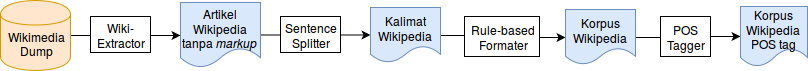
\includegraphics[width=\linewidth]{pics/Pic02-PreProcessingWikipedia}
    \caption{Pre-processing Data Wikipedia}
    \label{fig:preproses-wiki}
\end{figure}

Data XML yang diperoleh dari Wikipedia Dump diekstrak secara otomatis menggunakan WikiExtractor\footnote{github.com/attardi/wikiextractor/wiki}. WikiExtractor adalah program berbasis Python yang dibuat oleh Giuseppe Attardi dan Antonio Fuschetto. \textit{Tools} ini akan membersihkan artikel Wikipedia dari format MediaWiki \textit{markup language} (Gambar 3.2) sehingga dihasilkan korpus yang hanya berisi konten artikel saja. Program ini dapat diunduh dari Github dan dijalankan pada sistem operasi berbasis UNIX/Linux menggunakan perintah berikut. 

\begin{lstlisting}[caption={Penggunaan Wiki Extractor}, language=bash]
$ WikiExtractor.py xml-dump-file -o output-file
\end{lstlisting}

\noindent Jika tidak memberi spesifikasi opsi apapun, artikel yang dihasilkan membersihkan seluruh \textit{markup language} dan hanya menyimpan isi artikel tanpa disertakan informasi seperti kategori, riwayat, dan versi artikel.

%-----------------------------------------------------------------------------%
\subsection{Sentence Splitting}
%-----------------------------------------------------------------------------%
Korpus yang dihasilkan menghasilkan baris-baris yang merepresentasikan suatu paragraf dalam artikel Wikipedia. Pada penelitian kali ini, ingin dilihat relasi hipernim-hiponim antar dua kata pada kalimat yang sama. Untuk itu, perlu dilakukan proses \textit{sentence splitting} yang dapat memisahkan setiap kalimat dalam paragraf. Hasil dari proses tersebut adalah dokumen yang terdiri dari baris-baris yang merepresentasikan satu kalimat. 

Proses ini dilakukan dengan menggunakan program berbasis Perl yang telah dibuat sebelumnya oleh \cite{ken2016pengembangan} dari Fasilkom UI, Indonesia. Ditambah satu program yang dapat secara otomatis melakukan \textit{splitting} untuk seluruh dokumen dalam direktori. Berikut adalah contoh sebuah paragraf dalam artikel Wikipedia yang telah dibersihkan menggunakan WikiExtractor.

\begin{center}
\begin{tabular}{ | m{32em} | } 
\hline
Charles Anthony Johnson (3 Juni 1829 - 17 Mei 1917), kemudian dikenal sebagai Charles Brooke memerintah Sarawak sebagai Raja Putih kedua dari 3 Agustus 1868 hingga meninggal dunia. Dia menggantikan pamannya, James Brooke sebagai raja. \\ \hline 
\end{tabular}
\end{center}

\noindent Paragraf   di atas akan dimasukkan ke program \textit{sentence splitter}. Berikut adalah hasil yang diberikan dari proses tersebut.

\begin{center}
\begin{tabular}{ | m{32em} | } 
\hline
Charles Anthony Johnson (3 Juni 1829 - 17 Mei 1917), kemudian dikenal sebagai Charles Brooke memerintah Sarawak sebagai Raja Putih kedua dari 3 Agustus 1868 hingga meninggal dunia. \\ \hline 
Dia menggantikan pamannya, James Brooke sebagai raja. \\
\hline
\end{tabular}
\end{center}

%-----------------------------------------------------------------------------%
\subsection{Rule Based Formatter}
%-----------------------------------------------------------------------------%
Kalimat-kalimat yang terbentuk, selanjutnya diproses dengan program \textit{rule based formatter} sehingga membentuk korpus dengan format yang diingingkan. Penambahan aturan juga untuk mengurangi ambiguitas dan bentuk usaha membentuk \textit{pattern} yang lebih umum. Berikut adalah beberapa aturan tambahan untuk yang diberikan pada korpus Wikipedia.

\begin{enumerate}
  \item Menghilangkan frasa yang berada di dalam tanda kurung. \\
  Frasa yang terletak di dalam tanda kurung dapat dianggap sebagai penjelas kata atau frasa sebelumnya. Proses ini dilakukan agar dapat mengekstrak lebih banyak \textit{pattern} yang sama.
  \item Memisahkan simbol-simbol yang berhimpit pada awal dan akhir kata. \\
  Beberapa token yang dipisahkan oleh spasi dalam kalimat merupakan kata yang berhimpit dengan tanda baca. Untuk mempermudah proses selanjutnya yaitu \textit{sentence tagging}, dilakukan \textit{pre-processing} tambahan yaitu memisahkan simbol-simbol \textit{non-alphanumerical}.
  \item Memberi penanda awal kalimat dengan '{\tagStart}' dan akhir kalimat dengan '{\tagEnd}'. \\
  Pemberian simbol awal dan akhir kalimat memperjelas isi kalimat dan juga menunjang proses \textit{pattern extraction} dan \textit{pattern matching}.
\end{enumerate}

\noindent Dari contoh kalimat di atas, setelah melalui proses \textit{formatting} yang didefinisikan menghasilkan kalimat berikut.

\begin{center}
\begin{tabular}{ | m{32em} | } 
\hline
{\tagStart} Charles Anthony Johnson , kemudian dikenal sebagai Charles Brooke memerintah Sarawak sebagai Raja Putih kedua dari 3 Agustus 1868 hingga meninggal dunia . {\tagEnd} \\
\hline 
{\tagStart} Dia menggantikan pamannya , James Brooke sebagai raja . {\tagEnd} \\
\hline
\end{tabular}
\end{center}

%-----------------------------------------------------------------------------%
\subsection{POS Tagging Kalimat Wikipedia}
%-----------------------------------------------------------------------------%
Proses \textit{part-of-speech tagging} dilakukan pada korpus Wikipedia yang telah berbentuk kalimat dengan format yang didefinisikan. Pada penelitian ini, kelas kata yang menjadi pengamatan adalah \textit{noun} (NN) dan \textit{proper noun} (NNP), sehingga proses \textit{POS Tagging} perlu dilakukan untuk mengidentifikasi kata-kata tersebut. Proses ini dijalankan menggunakan program Stanford POS Tagger \citep{toutanova2003feature} dan sebuah model Bahasa Indonesia yang merupakan hasil penelitian sebelumnya \citep{dinakaramani2014designing}.  Setelah selesai melalui proses \textit{tagging} masih ditemui beberapa kesalahan \textit{tagging} untuk beberapa token. Hal ini menyebabkan ditambahkannya \textit{rule-based tagging} untuk memperbaik kata-kata yang sering salah. Selanjutnya dilakukan penyesuaian format sehingga korpus yang dihasilkan lebih rapi dan terstruktur. Berikut adalah contoh kalimat yang sudah melalui tahap \textit{POS Tagging}. Kalimat tersebut digunakan untuk proses \textit{pattern matching}.

\begin{center}
\begin{tabular}{ | m{32em} | } 
\hline
{\tagStart}\_X Charles\_NNP Anthony\_NNP Johnson\_NNP ,\_Z kemudian\_CC dikenal\_VB sebagai\_IN Charles\_NNP Brooke\_NNP memerintah\_VB Sarawak\_NNP sebagai\_IN Raja\_NNP Putih\_NNP kedua\_CD dari\_IN 3\_CD Agustus\_NNP 1868\_CD hingga\_IN meninggal\_VB dunia\_NN .\_Z {\tagEnd}\_X \\ \hline
\end{tabular}
\end{center}

%
%-----------------------------------------------------------------------------%
\section{Seed Builder}
%-----------------------------------------------------------------------------%
Proses pengumpulan \textit{seed} dibantu dengan \textit{resource} yang dimiliki WordNet Bahasa menggunakan \textit{tools} nltk. Proses pengumpulan diawali dengan mengambil seluruh lema Bahasa Indonesia yang dimiliki oleh korpus nltk. Setelah itu, ambil seluruh \textit{synset} yang mengandung lemma tersebut. Dari setiap \textit{synset}, ambil relasi hipernimnya. Dari setiap \textit{synset} hipernim, ambil lema Bahasa Indonesianya. Dilakukan pula filterisasi \textit{synset} ataupun lema untuk mengurangi ambiguitas. Untuk setiap \textit{synset} maupun lema yang diambil pada setiap tahapan, hanya boleh berasal dari kelas kata kerja (\textit{noun}). Setelah didapatkan, bentuk ke dalam pasangan \textit{tuple} biner. Berikut adalah

%--- kode seed builder ----- %
\begin{lstlisting}[caption={Algoritme pembentukan \textit{seed}}, language=bash]
buildSeed:
  ls = get_all_indonesian_lemma()
  for l in ls:
    syns = get_all_synsets(l)
    for s in syns:
      hs = get_all_hypernyms(s)
      for h in hs: 
        hls = get_lemmas(h)
        for hl in hls:
          filter(hl)
          print_seed(l, hl)
\end{lstlisting}

% Filterisasi Seed
Filterisasi dilakukan dengan tujuan mengurangi ambiguitas, namun tetap berusaha mendapatkan \textit{seed} sebanyak mungkin. Filterasisasi juga dilakukan untuk mendapatkan \textit{seed} awal yang diyakini benar dan berkualitas baik. Salah satu bagian terpenting proses ini adalah memasangkan hanya lema yang merupakan \textit{noun} ke lema yang juga adalah \textit{noun}. Jika kemungkinan lema tersebut tergolong ke dalam kelas kata bukan \textit{noun}, lema tidak diikutsertakan sebagai \textit{seed} awal.

Tantangan dalam proses ini adalah banyak ditemukan kasus dimana satu lema dikandung oleh lebih dari satu \textit{synset} atau satu \textit{synset} memiliki lebih dari satu \textit{synset} hipernim. Ambiguitas dalam kasus tersebut dapat mengurangi kualitas \textit{seed} yang dihasilkan. Mengatahui hal tersebut, dibuatlah dua pendekatan berbeda untuk proses filterisasi \textit{seed}.

Pendekatan pertama adalah tetap mengambil lemma yang sama pada \textit{synset} hipernim yang berbeda. Hal ini dilatarbelakangi adanya lema yang berasal dari \textit{synset} berbeda namun memiliki lema hipernim yang sama. Pada contoh (i), satu lema yang sama dimiliki oleh dua \textit{synset} yang berbeda namun kedua \textit{synset} tersebut memiliki \textit{synset} hipernim yang sama. Lema untuk kedua \textit{synset} hipernim juga sama sehingga tetap diikutsertakan sebagai \textit{seed}. Pada contoh (ii), satu lema berasal dari dua \textit{synset} yang berbeda dan dua \textit{synset} hipernim berbeda, namun ada lema yang sama yaitu 'laluan'. Sehingga pasangan `(pintu\_masuk;laluan)' tetap diikutsertakan sebagai \textit{seed}.

Pendekatan lainnya adalah dengan metode filterisasi yang \textit{strict}. Jika satu lema memiliki lebih dari satu \textit{synset} hipernim, maka lema tersebut dianggap ambigu dan langsung tidak diikutsertakan ke dalam \textit{seed} awal. Berdasarkan tabel contoh lema, \textit{synset}, dan hipernimnya, hanya contoh (i) yang diterima sebagai \textit{seed} karena \textit{synset} hipernim untuk lema tersebut sama. Sementara (ii) ditolak karena \textit{synset} hipernim berbeda.

\begin{center}
\begin{tabular}{ |c|m{30em}| } 
  \hline
  \multirow{2}{*}{i.} 
  & (paruh, Synset(beak.n.02)) => ([bibir, kuala, muara], Synset(mouth.n.02)) \\ 
  & (paruh, Synset(beak.n.01)) => ([bibir, kuala, muara], Synset(mouth.n.02)) \\ \hline
\multirow{2}{*}{ii.} 
  & (pintu\_masuk, Synset(entrance.n.01)) => ([akses, capaian, laluan], Synset(access.n.03)) \\ 
  & (pintu\_masuk, Synset(orifice.n.01)) => ([koridor, laluan, lorong], Synset(passage.n.07)) \\ \hline
\end{tabular}
\end{center}

\noindent Format penulisan $(l_1, S_1) => (ls_2, S_2)$ dibaca $l_1$ adalah lema hiponim, $S_1$ adalah \textit{synset} hiponim, $ls_2$ adalah himpunan lema hipernim, dan $S_2$ adalah \textit{synset} hipernim. 
%
%--------------------------- %
% \begin{figure}
%     \centering
%     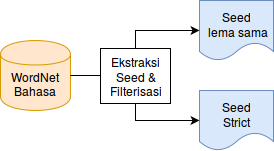
\includegraphics[scale=0.6]{pics/Pic02-SeedBuilder}
%     \caption{Proses Pembentukan \textit{Seed}}
%     \label{fig:seed-builder}
% \end{figure}

%
%-----------------------------------------------------------------------------%
\section{Sentence Tagging}
%-----------------------------------------------------------------------------%
Pada gambar \ref{fig:pattern-extraction} diperlihatkan bahwa tahap awal pembentukan \textit{pattern} adalah melakukan \textit{tagging} pasangan kata relasi ke dalam kalimat-kalimat Wikipedia. 

\begin{figure}
    \centering
    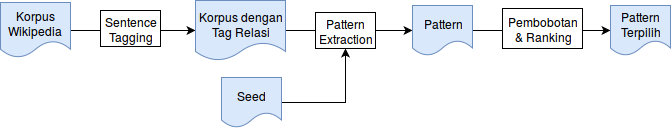
\includegraphics[width=\linewidth]{pics/Pic03-PatternExtraction}
    \caption{Proses Pembentukan \textit{Pattern}}
    \label{fig:pattern-extraction}
\end{figure}

\noindent Data yang digunakan untuk proses ini adalah korpus Wikipedia tanpa \textit{pos tag}. Beberapa tahapan dilakukan pada proses \textit{tagging sentence} dengan pasangan kata relasi adalah sebagai berikut.

\begin{enumerate}
  \item Dibaca seluruh pasangan kata relasi hipernim-hiponim.
  \item Untuk setiap kalimat pada korpus Wikipedia, di cek apakah kalimat tersebut mengandung kedua kata dalam pasangan kata relasi.
  \item Pengecekan dilakukan secara berulang untuk seluruh pasangan kata relasi karena terdapat kemungkinan satu kalimat mengandung lebih dari satu pasang kata relasi.
  \item Kata-kata yang merupakan bagian dari pasangan kata relasi kemudian diberi \textit{tag} sesuai relasinya dan disimpan ke dalam korpus berisi kalimat yang sudah memiliki \textit{tag} hiponim dan hipernim.
\end{enumerate}

Pada penelitian ini, satu kalimat yang telah di-\textit{tag} hanya mengandung tepat satu pasangan kata relasi. Untuk kasus khusus dimana suatu pasangan kata relasi terdiri dari suatu kata yang merupakan sub kata pasangannya, maka pasangan kata tersebut tidak diikutsertakan untuk menghindari ambiguitas. Contoh pasangan kata yang tidak diikutsertakan adalah $(ikan\,\,gurame;ikan)$ dimana kata 'ikan' terkandung dalam kedua kata relasi.

Berikut adalah contoh kalimat yang terbentuk dari proses \textit{sentence tagging}. Diberikan pasangan kata relasi hipernim-hiponim $(fermion;partikel)$ dan $(boson;partikel)$ serta kalimat  '{\tagStart} seluruh partikel dasar adalah boson atau fermion . {\tagEnd}'. Hasil proses \textit{sentence tagging} adalah sebagai berikut.
\begin{itemize}
  \item {\tagStart} seluruh {\tagHypernym}partikel{\tagHypernym} dasar adalah boson atau {\tagHyponym}fermion{\tagHyponym} . {\tagEnd}
  \item {\tagStart} seluruh {\tagHypernym}partikel{\tagHypernym} dasar adalah {\tagHyponym}boson{\tagHyponym} atau fermion . {\tagEnd}
\end{itemize}
%
% %--- kode sentence tagging ----- %
% \begin{lstlisting}[caption={Algoritme \textit{sentence tagging}}, language=bash]
% tagAll:
%   seeds = load_all_seeds()
%   foreach sentence in sentences:
%     tagSentence(sentence, seeds)
%
% tagSentece(sentence, seeds):
%   foreach seed in seeds:
%     if (sentence.contains(seed.hypernym) && sentence.contains(seed.hyponym)):
%       put_tag_hyponym()
%       put_tag_hypernym()
%       save_sentence()
% \end{lstlisting}
% %------------------------------ %

%
%-----------------------------------------------------------------------------%
\section{Pattern Extraction}
%-----------------------------------------------------------------------------%
Setelah mendapatkan kalimat-kalimat yang telah di-\textit{tag} dengan kata relasi, ingin dicari \textit{pattern} yang dapat digunakan untuk menambah jumlah relasi kata. Gambar \ref{fig:pattern-extraction} menunjukan bahwa kalimat-kalimat tersebut selanjutnya masuk ke dalam proses \textit{pattern extraction}. Pada penelitian ini, diusulkan pembuatan \textit{pattern} menggunakan \textit{standard tree} dengan beberapa modifikasi. Proses ini diimplementasi secara mandiri menggunakan program Java dengan mengikuti algoritma pemebentukkan \textit{tree} sederhana.

Suatu \textit{\textit{node}} merepresentasikan kata dalam kalimat dan dari satu kalimat terbentuk sebuah cabang dalam \textit{tree}. \textit{Node} menyimpan beberapa informasi seperti nama \textit{\textit{node}}, \textit{parent}, \textit{childs}, dan informasi identitas tambahan seperti apakah \textit{\textit{node}} tersebut merupakan relasi (hipernim atau \textit{hyponym}) dan apakah \textit{\textit{node}} tersebut merupakan \textit{leaf}. Untuk kata yang merupakan kata relasi, \textit{\textit{node}} menyimpan informasi jenis relasi beserta \textit{list} dari kata yang merupakan bagian dari relasi tersebut. 

Sebagai contoh jika terdapat beberapa \textit{sequnce} kalimat yang akan dibentuk ke dalam \textit{tree} sebagai berikut menghasilkan \textit{tree} seperti yang dapat dilihat pada gambar \ref{fig:contoh-ptree}.

K1: {\tagHyponym}piano{\tagHyponym} adalah {\tagHypernym}alat musik{\tagHypernym}.

K2: {\tagHyponym}Van Gogh{\tagHyponym} adalah seorang {\tagHypernym} pelukis{\tagHypernym}.

K3: {\tagHyponym}kucing{\tagHyponym} adalah {\tagHypernym}binatang{\tagHypernym}.

K4: {\tagHyponym}sepak bola{\tagHyponym} adalah {\tagHypernym} olahraga{\tagHypernym}.

\begin{figure}
    \centering
    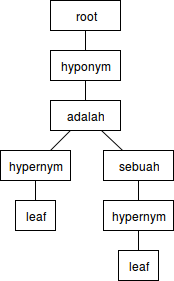
\includegraphics[scale=0.7]{pics/contoh-patterntree}
    \caption{Contoh \textit{pattern tree} yang terbentuk}
    \label{fig:contoh-ptree}
\end{figure}

\noindent Dari \textit{tree} di atas, terdapat dua \textit{pattern} utama yang merepresentasikan korpus kalimat yaitu `{\tagHyponym} adalah {\tagHypernym}' dan `{\tagHyponym} adalah seorang {\tagHypernym}'.

%-----------------------------------------------------------------------------%
\subsection{Informasi dalam Pattern}
%-----------------------------------------------------------------------------%
Satu \textit{pattern} tidak hanya menyimpan informasi \textit{sequence} kata yang merepresentesaikan \textit{pattern} tersebut, namun juga beberapa informasi tambahan lainnya. Informasi-informasi lain tersebut adalah jumlah kemunculan dalam korpus, \textit{seed} unik yang membentuk \textit{pattern}, dan kalimat unik yang membentuk \textit{pattern}. Informasi-informasi tersebut digunakan untuk pembentukan vektor \textit{pattern}, pemberian bobot \textit{pattern}, dan melakukan \textit{sorting} untuk mendapatkan \textit{pattern} terbaik.

%-----------------------------------------------------------------------------%
\subsection{Pattern Tree}
%-----------------------------------------------------------------------------%
\textit{Pattern Tree} adalah sebuah \textit{tree} yang menyimpan seluruh \textit{pattern} yang dihasilkan dari korpus, seperti yang telah dipaparkan pada gambar \ref{fig:contoh-ptree}. Dalam pembuatan \textit{pattern tree}, tidak perlu menyimpan seluruh kata dalam kalimat. Hanya \textit{sequence} kata tertentu saja yang dianggap dapat menghasilkan \textit{pattern} yang baik untuk diikutsertakan. Maka dari itu, perlu diketahui \textit{sequence} kata dalam kalimat yang cocok digunakan sebagai \textit{pattern}. Berikut adalah tiga pendekatan yang digunakan dalam penelitian ini dengan contoh kalimat dasarnya yaitu `{\tagStart} {\tagHyponym}singa{\tagHyponym} adalah {\tagHypernym}kucing{\tagHypernym} yang berukuran besar . {\tagEnd}'.

\begin{enumerate}
  \item Hanya memperhatikan kata yang berada diantara pasangan kata relasi. \\
  Pada kasus ini, hanya ingin dilihat kata-kata yang berada diantara kata yang merupakan hipernim-hiponim atau hipernim-hiponim. Kata-kata diantara dua relasi dapat dianggap paling dekat jika ingin mencari \textit{memisahkan} setiap relasi tersebut. Pada contoh diatas, \textit{sequence} kata yang dihasilkan adalah `{\tagHyponym}singa{\tagHyponym} adalah {\tagHypernym}kucing{\tagHypernym}'
  \item Mengikutsertakan $n$ kata sebelum kata relasi pertama. \\
  Beberapa kata berbasis Perl sebelum program dapat memberikan informasi untuk yang dapat meningkatkan kualitas satu program. Pada contoh kalimat diatas dengan $(n=1)$, \textit{sequence} kata yang dihasilkan adalah `{\tagStart} {\tagHyponym}singa{\tagHyponym} adalah {\tagHypernym}kucing{\tagHypernym}'
  \item Mengikutsertakan $n$ kata setelah kata relasi terakhir. \\
  Tipe ini sama dengan sebelumnya, namun dilihat pengaruh kata-kata yang mengikuti kata relasi. Pada contoh kalimat diatas dengan $(n=1)$, \textit{sequence} kata yang dihasilkan adalah `{\tagHyponym}singa{\tagHyponym} adalah {\tagHypernym}kucing{\tagHypernym} yang'
\end{enumerate}

Suatu kalimat akan di-\textit{parse} ke dalam bentuk \textit{array} yang elemennya merepresentasikan kata dalam kalimat. Proses \textit{parsing} dilakukan berdasarkan spasi antar kata. Dari \textit{array} yang terbentuk, dicari bagian-bagian yang akan dimasukkan ke dalam \textit{pattern tree} sesuai dengan pendekatan yang dipilih. Jika hanya memperhatikan kata diantara pasangan kata relasi maka bagian-bagian lain tidak masuk ke dalam \textit{pattern tree}. Begitu jika dipilih pendekatan dengan $n$ kata sebelum atau setelah pasangan kata. Dari \textit{pattern tree} yang terbentuk, dapat didaftarkan seluruh \textit{pattern} serta bobot untuk \textit{pattern} tersebut. Kode \ref{code:pembentukan-ptree} menunjukan secara rinci proses penambahan suatu \textit{pattern} ke dalam \textit{pattern tree}.

% --- kode pattern extraction: createPatternTree ---  
\begin{lstlisting}[caption={Penambahan \textit{pattern} ke dalam \textit{pattern tree}}, language=bash, label={code:pembentukan-ptree}]
sentence = #kalimat baru yang akan dimasukkan
type = #pendekatan yang dipilih
ptree = #pattern tree yang sudah terbentuk

addNewPattern(sentence, type, ptree):
  sentence_arr = split(sentence, `` '')
  index = getIndexToken(sentence_arr, type)
  addPattern(ptree, sentence_arr, index)

getIndexToken(sentence_arr, type):
  sentence_arr = tokenize_sentence(sentence)
  index = (start, end)
  if (type == inbetween):
    for(i = 0..sentence_arr.size()):
      if (token == relation):
        if (!start) start = i
        else end = i
  else if (type == n before):
    index = getIndexToken(sentence_arr, inbetween)
    if (index.start - n >= 0)
      index.start -= n
    else index.start = 0
  else if (type == n after):
    index = getIndexToken(sentence_arr, inbetween)
    if (index.end + n < sentence_arr.size())
      index.end += n
    else index.end = sentence_arr.size()
  return index
\end{lstlisting}
% -------------------------------------------------- %

%-----------------------------------------------------------------------------%
\subsection{Vektor Pattern}
%-----------------------------------------------------------------------------%
Suatu \textit{pattern} dapat direpresentasikan menjadi vektor berdasarkan nilai-nilai yang dimilikinya. Vektor ini dimanfaatkan untuk melakukan pengurutan terhadap seluruh \textit{pattern} yang dihasilkan. Selain itu, nilai-nilai pada vektor \textit{pattern} juga digunakan untuk melakukan filterisasi. Fitur utama pada vektor \textit{pattern} diambil dari informasi yang disimpan \textit{pattern}, yaitu total kemunculan \textit{pattern}, jumlah \textit{seed} unik, dan jumlah kalimat unik yang membentuk \textit{pattern} tersebut. Fitur lainnya adalah hasil kombinasi perbandingan antar nilai-nilai utama, yaitu nilai perbandingan antara jumlah \textit{seed} unik dibagi jumlah kalimat unik, nilai perbandingan antara jumlah \textit{seed} untuk dibagi total kemunculan, dan nilai perbandingan antara jumlah kalimat unik dibagi total kemunculan.

Berikut adalah contoh vektor \textit{pattern} yang dihasilkan.
\begin{equation}
<start>\,\,<hyponym>\,\,adalah\,\,<hypernym>\,\,;\,\,96\,\,87\,\,95\,\,0.92\,\,0.91\,\,0.99
\end{equation}
\begin{itemize}
  \item \textit{pattern} leksikal yang dihasilkan = \[<start>\,\,<hyponym>\,\,adalah\,\,<hypernym>\]
  \item jumlah total kemunculan \textit{pattern} = 96
  \item jumlah pasangan kata relasi unik yang membentuk \textit{pattern} = 87
  \item jumlah kalimat unik yang membentuk \textit{pattern} = 95
  \item perbandingan nilai pasangan kata unik dengan kalimat unik = 0.92
  \item perbandingan nilai pasangan kata unik dengan total kemunculan = 0.91
  \item perbandingan nilai kalimat unik dengan total kemunculan = 0.99
\end{itemize}

%-----------------------------------------------------------------------------%
\subsection{Validasi Pattern}
%-----------------------------------------------------------------------------%
Setelah terbentuk \textit{pattern tree}, perlu didaftar seluruh \textit{pattern} yang dihasilkan. Proses pembentukan \textit{pattern} cukup dengan menelusuri \textit{path} dari \textit{node leaf} hingga \textit{root}. \textit{Pattern} yang dihasilkan berjumlah banyak, sayangnya tidak seluruh \textit{pattern} yang dihasilkan berkualitas baik. Untuk mengurangi jumlah \textit{pattern} yang kurang baik, dilakukan proses filterisasi. Beberapa aturan yang harus dipenuhi agar suatu \textit{pattern} diterima adalah sebagai berikut.

\begin{itemize}
  \item Harus ada minimal satu kata diantara dua kata relasi. \\
  Banyak kasus dimana dua kata relasi hanya dipisahkan oleh spasi. \textit{Pattern} yang hanya mengandung spasi tidak memberikan informasi apapun karena simbol spasi dalam Bahasa Indonesia digunakan sebagai pemisah antar kata. Sebagai contoh kalimat hasil \textit{tagging} `{\tagStart} semua jenis {\tagHypernym}ular{\tagHypernym} {\tagHyponym}beludak{\tagHyponym} memiliki taring yang panjang {\tagEnd}' tidak akan menghasilkan \textit{pattern} yang \textit{valid}.
  \item Nilai dalam vektor \textit{pattern} harus memenuhi nilai \textit{threshold} yang didefinisikan. \\
  Nilai perbandingan antara jumlah \textit{seed} unik dibagi jumlah kalimat unik lebih dari 0.5. Nilai perbandingan antara jumlah \textit{seed} unik dibagi total kemunculan lebih dari 0.2. Nilai perbandingan antara jumlah kalimat unik dibagi total kemunculan harus lebih dari 0.7. Ketiga nilai \textit{threshold} tersebut didefinisikan mandiri berdasarkan pengamatan dari nilai-nilai pada vektor \textit{pattern}. Nilai tersebut mengeliminasi sejumlah \textit{pattern} yang terbentuk dari banyak kalimat namun variasi \textit{seed} yang menghasilkannya sedikit.
\end{itemize}

%-----------------------------------------------------------------------------%
\subsection{Pembentukan \textit{Pattern} Unik}
%-----------------------------------------------------------------------------%
\textit{Pattern} yang dihasilkan dari tahap ini harus unik sehingga tidak terjadi ambiguitas jika hendak digunakan. Pada masa awal pengembangan, masalah yang muncul pada \textit{pattern} yang dihasilkan adalah adanya \textit{pattern} yang posisi hipernim-hiponimnya saling berkebalikan. Sebagai contoh beberapa \textit{pattern} ambigu yang dihasilkan seperti (i) {\tagHyponym} adalah {\tagHypernym}, (ii) {\tagHypernym} adalah {\tagHyponym}, (iii) {\tagHypernym} dan {\tagHyponym}, dan (iv) {\tagHyponym} dan {\tagHypernym}. Kata-kata pada kalimat yang menempati posisi hipernim-hiponim tersebut nantinya digantikan dengan kata yang kemunculannya sesuai dengan \textit{pattern} yang diberikan. Sehingga perlu ada strategi tambahan untuk mengatasi masalah tersebut.

Strategi yang diusulkan dalam penelitian ini untuk mengatasi masalah ambiguitas antar \textit{pattern} adalah membangun suatu arsitektur yang dapat mengidentifikasi dan menyelesaikan. Berikut adalah tahapan yang dilakukan untuk memastikan bahwa \textit{pattern} yang dihasilkan adalah unik.

\begin{enumerate}
  \item Dicari \textit{pattern} dengan pendekatan hanya memperhatikan kata-kata diantara pasangan kata relasi.
  \item \textit{Pattern} yang dihasilkan, dibandingkan satu dengan yang lain. Jika terdapat \textit{pattern} mengandung \textit{tag} hipernim-hiponim yang saling terbalik, \textit{pattern} yang bersangkutan dikeluarkan dari daftar \textit{pattern} unik untuk kemudian dievaluasi ulang.
  \item Proses evaluasi ulang dilakukan menggunakan pendekatan pembuatan \textit{pattern} lainnya yaitu dengan memperhatikan $n$ kata sebelum dan setelah kata hipernim-hiponim. Hasil dari kedua pendekatan digabung dan dicek apakah \textit{pattern} tersebut dibutuhkan. Suatu \textit{pattern} dinyatakan dibutuhkan jika \textit{substring} dari \textit{pattern} tersebut termasuk dalam \textit{list pattern} yang membutuhkan evaluasi ulang.
  \item Proses evaluasi dilakukan secara berulang dari hingga iterasi ke-$n$.
\end{enumerate}

\noindent Setelah melakukan tahapan di atas, tidak ada lagi kasus posisi relasi saling tertukar dari \textit{pattern} yang dihasilkan. Daftar \textit{pattern} unik yang dihasilkan kemudian diurutkan berdasarkan bobot sebelum ditampilkan.
%
% % --- kodepattern extraction: patternUnik --- %
% \begin{lstlisting}[caption={Algoritme pembentukan \textit{pattern unik}}, language=bash]
% patternUnik():
%   patternunik; patterntmp;
%   patterns = getPattern(inbetween)
%   unikfy(patterns)
%   i = 0;
%   while (patterntmp is not empty && i < 3):
%     before-patterns = getPattern(i-before)
%     after-patterns = getPattern(i-after)
%     hasil = cekNeeded(before-patterns, after-patterns)
%     unikfy(hasil)
%   return patternunik

% unikfy(patterns):
%   mappatterns;
%   foreach pattern in patterns:
%     pk = pattern.getKey()
%     if (mappatterns.containsKey(pk)):
%       mappatterns.get(pk).add(pattern)
%     else:
%       mappatterns.put(pk, List.add(pattern))
%   foreach pk in mappatterns:
%     if mappatterns.get(pk).size() > 0:
%       patterntmp.add(pk)
%     else 
%       patternunik.add(mappatterns.get(pk))
% \end{lstlisting}
% % -------------------------------------------------- %

%-----------------------------------------------------------------------------%
\subsection{Pengurutan Pattern}
%-----------------------------------------------------------------------------%
Setelah terbentuk \textit{pattern} yang sesuai, dilakukan proses pengurutan (\textit{sorting}) untuk mengetahui \textit{pattern} mana yang terbaik berdasarkan informasi dalam vektor \textit{pattern}. Proses pengurutan dilakukan dengan membandingkan satu \textit{pattern} dengan yang lain, dengan tahapan sebagai berikut.
\begin{enumerate}
  \item Semakin besar jumlah kalimat unik yang membentuk \textit{pattern}.
  \item Semakin besar nilai perbandingan antara jumlah \textit{seed} unik yang membentuk \textit{pattern} dengan jumlah kalimat unik yang membentuk \textit{pattern}.
  \item Semakin sedikit jumlah token dalam \textit{pattern} jika di-\textit{parse} menggunakan spasi.
\end{enumerate}

%
%-----------------------------------------------------------------------------%
\section{Pattern Matching}
%-----------------------------------------------------------------------------%
Proses ekstraksi \textit{pair} baru dilakukan dengan menggunakan metode \textit{pattern matching} seperti yang dapat dilihat pada gambar \ref{fig:pattern-matching}. \textit{Pattern} yang terbentuk dari proses \textit{pattern extraction} digunakan untuk menambah jumlah pasangan kata relasi dengan dilakukan proses \textit{pattern matching} terhadap korpus Wikipedia. Proses \textit{pattern matching} dilakukan menggunakan algoritma \textit{Suffix Tree} dengan modifikasi. Implementasi dilakukan secara mandiri menggunakan program berbasis Java.

\begin{figure}
    \centering
    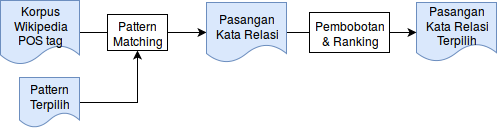
\includegraphics[scale=0.6]{pics/Pic04-PatternMatching}
    \caption{Proses ekstraksi \textit{pair}}
    \label{fig:pattern-matching}
\end{figure}

Pembentukan \textit{suffix tree} mirip seperti pembentukan \textit{pattern tree} yaitu diawali dengan melakukan \textit{parsing} sehingga satu kalimat terepresentasi dalam bentuk \textit{array}. Dari \textit{array} yang dihasilkan, dibentuk sebuah \textit{suffix tree} yang merepresentasikan kalimat tersebut. Sebuah \textit{node} dalam \textit{tree} merepresentasikan satu kata dalam kalimat. \textit{Suffix tree} selanjutnya dicocokan dengan \textit{pattern} yang diberikan. Jika terdapat \textit{path} dalam \textit{tree} yang sesuai dengan \textit{pattern}, dibentuk \textit{pair} yang merepresentasikan pasangan kata relasi hipernim-hiponim yang dihasilkan. Selain kata hipernim-hiponim, \textit{pair} juga menyimpan informasi lain seperti total total dokumen unik, daftar kalimat unik, dan daftar \textit{pattern} unik yang menghasilkan \textit{pair} tersebut. Berikut adalah tahapan yang dilakukan program jika diberikan satu kalimat dan satu \textit{pattern}.

\begin{enumerate}
  \item Kalimat masukan dibentuk menjadi suatu \textit{suffix tree}.
  \item \textit{Pattern} masukan ditokenisasi ke dalam bentuk \textit{list} 
  kata. \textit{Pattern} pasti mengandung token {\tagHypernym} dan {\tagHyponym}, selanjutnya disebut token relasi.
  \item Jika ditemukan token relasi pada daftar token \textit{pattern} yang sedang dievaluasi, maka \textit{node} yang dikunjungi disimpan sementara sesuai dengan relasinya.
  \item Jika token bukan token relasi, maka di evaluasi apakah token sama denga  \textit{node} yang dikunjungi. Jika sama maka proses evaluasi dilanjutkan, namun jika berbeda maka \textit{pattern} tidak cocok.
  \item Jika seluruh token \textit{pattern} telah dievaluasi dan tidak mengalami kegagalan, maka dianggap berhasil dan kata yang terekstrak disimpan dalam bentuk \textit{pair}.
\end{enumerate}

Pada masa awal pengembangan, masalah pertama yang ditemukan adalah banyaknya \textit{pair} yang salah satu atau kedua kata relasinya tidak teramasuk dalam kelas kata benda. Beberapa \textit{pair} yang salah diantaranya $(Menoitios;salah)$ dimana 'salah' adalah \textit{adjective} dan $(saya,gitaris)$ dimana 'saya' adalah preposi. Untuk itu diputuskan menggunakan korpus Wikipedia yang sudah melalui tahap POS Tagging. \textit{POS tag} pada setiap kata dalam kalimat membatasi proses \textit{pattern matching} hanya akan mengekstrak \textit{pair} yang kedua katanya berada dalam kelas kata benda (\textit{noun} atau \textit{proper noun}). 

Masalah lain yang ditemukan adalah jika kata yang ingin diekstrak merupakan \textit{multi token}. \textit{Pair} kurang baik yang dihasilkan sebelum mengatasi masalah ini diantaranya adalah $(bola;olahraga)$ yang seharusnya $(sepak\,\,bola;olahraga)$, $(Serikat;negara)$ yang seharusnya $(Amerika\,\,Serikat;negara)$, dan $(Monterrey,ibu)$ yang seharusnya $(Monterrey;ibu\,\,kota)$. Solusi yang digunakan untuk mengatasi masalah ini adalah dengan mengasumsikan kata-kata berurutan yang tergolong dalam kelas kata yang sama dalam suatu kalimat merupakan \textit{multi token}. \textit{Multi token} disimpan dalam satu \textit{node} pada pembentukan \textit{suffix tree}.

% pembentukan multi token (parsing kalimat)
Untuk dapat mengidentifikasi \textit{multi token}, penyesuaian dilakukan pada tahap \textit{parsing} kalimat menjadi \textit{array}. Satu token akan bergabung dengan token sebelumnya jika memiliki \textit{pos tag} yang sama. Proses ini menghasilkan satu \textit{array} yang merepresentasik kalimat dimana setiap elemen dalam \textit{array} dapat merupakan \textit{single token} maupun \textit{multi token}. Kode \ref{code:pembentukan-stree} memaparkan proses pembentukan \textit{array} yang digunakan untuk membangun \textit{suffix tree}.

\begin{lstlisting}[caption={Proses \textit{parsing} kalimat menjadi \textit{array}}, language=bash, label={code:pembentukan-stree}]
sentence = #kalimat yang akan dievaluasi

getSentenceArray(sentence):
  tmp_arr = split(sentence, `` '')
  sentence_arr = []
  prev = null
  i = 0
  for s in sentence_arr:
    if (sentence.tag == prev.tag):
      sentence_arr[i-1] += `` '' + s
    else
      sentence_arr[i].add(s)
      i++
    prev = s
  return sentence_arr
\end{lstlisting}
%
% % --- kode pattern matching --- %
% \begin{lstlisting}[caption={Algoritme ekstraksi \textit{pair}}, language=bash]
% main:
%   patterns = loadAllPatterns()
%   openFiles()
%   for sentence in sentences:
%     matchAllPattern(sentence, patterns)

% matchAllPattern(sentence, patterns):
%   suffix_tree = buildTree(sentence)
%   foreach pattern in patterns:
%     matchTree(suffix_tree, pattern)
  
% buildTree(sentence):
%   tokens = buildSequence(sentence)
%   suffix_tree;
%   for(i = 0..tokens.size()):
%     addSequence(suffix_tree, tokens, i)
%   return suffix_tree;
% addSequence(suffix_tree, tokens, i):
%   node = suffix_tree.root
%   for (j=i..tokens.size()):
%     if (!node.childs.contains(tokens[j])):
%       node = node.childs.add(tokens[j])
%     node = node.childs.get(tokens[j])

% matchTree(stree, pattern):
%   foreach child in stree.root.childs:
%     recursiveMatch(pattern, 0, child, ``'', ``'')
% recursiveMatch(pattern, i, node, hype, hypo):
%   if (i >= pattern.size() && hype && hypo):
%     pair = createPair(hype, hypo)
%     savePair(pair)
%   else:
%     cek = pattern[i]
%     if (cek == ``hypenrym'' && cek.tag == (NN|NNP)):
%       hype = cek
%     else if (cek == ``hyponym'' && cek.tag == (NN|NNP)):
%       hypo = cek
%     else 
%       if (cek != node.name) return
%     foreach c in node.childs:
%       recursiveMatch(pattern, i+1, c, hype, hypo)
% \end{lstlisting}
% % -------------------------------------------------- %

%-----------------------------------------------------------------------------%
\subsection{Vektor Pair}
%-----------------------------------------------------------------------------%
Suatu \textit{pair} dapat direpresentasikan ke dalam bentuk vektor berdasarkan nilai-nilai yang dimilikinya. Nilai-nilai fitur yang dimiliki oleh sebuah \textit{pair} adalah total kemunculan \textit{pair}, total dokumen yang membentuk \textit{pair}, jumlah \textit{pattern} unik, dan jumlah kalimat unik. Untuk memperkaya fitur \textit{pair}, dilakukan pula Word Embedding. Nilai \textit{similarity} antar dua kata relasi ditambahkan sebagai sebagai salah satu fitur.

%-----------------------------------------------------------------------------%
\subsection{Filterisasi Pair}
%-----------------------------------------------------------------------------%
\textit{Pair} baru yang dihasilkan untuk proses ini berjumlah sangat banyak, namun tidak semua \textit{pair} yang dihasilkan adalah benar merupakan pasangan kata yang memiliki relasi semantik hipernim-hiponim. Beberapa \textit{pair} kebetulan terekstrak akibat memenuhi \textit{pattern} leksikal yang sama dengan salah satu \textit{pattern} yang digunakan. Untuk mengeliminasi data yang tidak diyakini benar, dilakukan proses filterisasi sederhana terhadap setiap \textit{pair} yang dihasilkan. \textit{Pair} diyakini tidak terbentuk secara kebetulan jika terdapat lebih dari satu \textit{pattern} yang mengekstrak \textit{pair} tersebut. 

Setelah mengeliminasi \textit{pair} yang hanya terbentuk dari satu \textit{pattern}, selanjutnya dilakukan pembobotan menggunakan rumus \ref{eq:bobot-pair}. Jika nilai bobot melebihi \textit{threshold}, maka \textit{pair} dimasukkan ke dalam korpus pasangan kata relasi. Nilai \textit{threshold} sendiri menjadi salah satu masukan dalam parameter eksperimen.

\begin{equation}
\label{eq:bobot-pair}
Bobot = (\frac{jumlah\,\,pattern\,\,pembentuk\,\,pair}{jumlah\,\,pattern\,\,digunakan} + similarity\,\,score)/2
\end{equation}

\noindent \textit{Pair} yang lolos filterisasi akan bergabung ke dalam korpus pasangan kata relasi semantik hipernim-hiponim.
%
% %-----------------------------------------------------------------------------%
% %\subsection{Pengurutan Pair}
% %-----------------------------------------------------------------------------%
% %Pada saat ditampilkan, \textit{pair} diurutkan untuk mengetahui \textit{pair} mana yang diyakini paling benar. Proses pengurutan dilakukan berdasarkan beberapa tahap, yaitu 
% % Semakin besar jumlah \textit{pattern} unik yang menghasilkan \textit{pair}.
% % Semakin besar jumlah kalimat untuk yang menghasilkan \textit{pair}.

%
%-----------------------------------------------------------------------------%
\section{Pemodelan Word Embedding}
% TODO: tambahin penjelasan mengenai parameter2 gensim
%-----------------------------------------------------------------------------%
Untuk menambah fitur pada vektor \textit{pair} yang dapat menunjang proses evaluasi, dilakukan Word Embedding. Implementasinya menggunakan model Word2Vec berbasis Python. Proses ini dibuat secara otomatis dengan hanya memberi masukan dokumen Bahasa Indonesia berukuran besar. Dalam penelitian ini, dokumen Bahasa Indoensia yang digunakan adalah korpus Wikipedia yang telah di proses membentuk kalimat.

Model dibuat memanfaatkan korpus Wikipedia yang telah melalui proses POS Tagging. Korpus tersebut diolah sedemikian sehingga kata-kata yang dianggap \textit{multi word}, memiliki kelas kata sama berurutan, digabung dengan simbol garis  awah ('\_'). Hal ini dilatarbelakangi atas hasil \textit{pair} yang banyak merupakan\textit{multi word}. Jika hal ini tidak dilakukan, maka akan banyak kata yang tidak ditemukan dalam \textit{dictionary} yang dihasilkan model \textit{word embedding}. Kode \ref{code:model-we} menunjukan proses pembuatan model \textit{word embedding}.

\begin{lstlisting}[caption={Kode pembangunan model \textit{word embedding}}, language=bash, label={code:model-we}]
sentences = #kumpulan kalimat yang menjadi model

import gensim

min_count = 1 #jumlah minimum kata
size = 123 #panjang vektor
window = 5 #ukuran window
model = gensim.models.Word2Vec(sentences, min_count=1, size=123, window=5);

model.save(nama_berkas)
\end{lstlisting}

Model yang terbentuk, digunakan untuk memberi nilai \textit{similarity} antara kata hipernim-hiponim dalam satu \textit{pair}. Proses pencarian nilai \textit{similarity} dilakukan secara kolektif untuk setiap iterasi. Model yang terbentuk dibaca kemudian dicari \textit{similarity} untuk setiap pasang kata relasi hipernim-hiponim. Hal ini diharapkan dapat memberi informasi lebih terhadap kualitas \textit{pair} yang dihasilkan.
